\documentclass[10pt]{article}
\usepackage[margin=1in, paperwidth=8.5in, paperheight=11in]{geometry}
\usepackage{ifpdf,amsmath, amssymb, comment, color, graphicx, stmaryrd,setspace,enumitem,tikz, fancyhdr, wrapfig, textcomp, units, mathptmx, siunitx, multicol}

\setlength{\headheight}{14.5pt}
\newcommand{\Q}{\mathbb{Q}}
\newcommand{\R}{\mathbb{R}}
\newcommand{\Z}{\mathbb{Z}}
\newcommand{\vu}{\mathbf{u}}
\newcommand{\vv}{\mathbf{v}}
\newcommand{\vw}{\mathbf{w}}
\newcommand{\vi}{\mathbf{i}}
\newcommand{\vj}{\mathbf{j}}
\newcommand{\vk}{\mathbf{k}}
\newcommand{\vn}{\mathbf{n}}
\newcommand{\vr}{\mathbf{r}}
\newcommand{\va}{\mathbf{a}}
\newcommand{\vF}{\mathbf{F}}
\newcommand{\vL}{\mathbf{L}}
\newcommand{\vT}{\mathbf{T}}
\newcommand{\vN}{\mathbf{N}}
\newcommand{\proj}{\operatorname{proj}}
\newcommand{\orth}{\operatorname{orth}}
\newcommand\dotp[1][.5]{\,\mathbin{\vcenter{\hbox{\scalebox{#1}{$\bullet$}}}}\,}

% Solution text is in red. If you want the solutions to show, remove the \iffalse from the definition of the \red command.
%\newcommand{\red}[1]{ %\iffalse
%	\textcolor{red}{#1} }%\fi}

\newenvironment{red}{\color{red}}{\ignorespacesafterend}
\newcommand{\blue}[1]{\textcolor{blue}{#1}}
\newcommand{\green}[1]{\textcolor{green}{#1}}
\renewcommand{\section}[1]{\begin{center} \textbf{#1} \\\end{center}}
%
\hyphenpenalty=5000
\setlength{\parindent}{0in}
%\oddsidemargin=-.25in
\allowdisplaybreaks
\pagestyle{fancy}
\renewcommand{\headrulewidth}{0pt}
\lhead{MATH 203}
\rhead{Spring 2020}
%\lfoot{\copyright\ CLEAR Calculus 2010}
\cfoot{}

\begin{document}
%


%\onehalfspacing
\allowdisplaybreaks
%##################################################################
\section{PS\#7 - Partial derivatives - \red{Answer key} }

\begin{enumerate}[leftmargin=0pt]
\item (Activity 10.2.4) The speed of sound $C$ traveling through ocean water is a function of temperature, salinity and depth. It may be modeled by the function
\begin{equation*}
C=1449.2+4.6T-0.055T^2+0.00029T^3+(1.34-0.01T)(S-35)+0.016D.
\end{equation*}
Here $C$ is the speed of sound in meters/second, $T$ is the temperature in degrees Celsius, $S$ is the salinity in grams/liter of water, and $D$ is the depth below the ocean surface in meters.
\begin{enumerate}
    \item State the units in which each of the partial derivatives, $C_T$, $C_S$, and $C_D$, are expressed and explain the physical meaning of each.
    
    \begin{red}
    $C_T$ is measured in $\dfrac{\textrm{m/s}}{^\circ C}$, and it tells us how much the speed of sound in water changes as the temperature changes.
    
    $C_S$ is measured in $\dfrac{\textrm{m/s}}{\textrm{gm/L}}$, and it tells us how much the speed of sound in water changes as the salinity changes.
    
    $C_D$ is measured in $\dfrac{\textrm{m/s}}{\textrm{m}}$, and it tells us how much the speed of sound in water changes as the depth changes.
    \end{red}
    \item Find the partial derivatives $C_T$, $C_S$, and $C_D$. 
    
    \begin{red}
    \[C_T = 4.6 - 0.11 T + 0.00087 T^2 -0.01(S-35) \]
    \[C_S = 1.34-0.01T \]
    \[C_D = 0.016\]
    \end{red}
    \item Evaluate each of the three partial derivatives at the point where $T=10$, $S=35$ and $D=100$. What does the sign of each partial derivative tell us about the behavior of the function $C$ at the point $(10, 35, 100)$?
    
    \begin{red}
    $C_T(10, 35, 100) = 3.587$ -- so the speed of sound \textbf{increases} as the temperature goes up from this point.
    
    $C_S(10, 35, 100) = 1.24$ -- so the speed of sound \textbf{increases} as the salinity goes up from this point.
    
    $C_D(10, 35, 100) = 0.016$ -- so the speed of sound goes \textbf{up} as the depth increases from this point.
    \end{red}
\end{enumerate}
\item (Activity 10.2.5) The wind chill, as frequently reported, is a measure of how cold it feels outside when the wind is blowing. In the table below, the wind chill $w$, measured in degrees Fahrenheit, is a function of the wind speed $v$, measured in miles per hour, and the ambient air temperature $T$, also measured in degrees Fahrenheit. We thus view $w$ as being of the form $w=w(v,T).$
\[\begin{array}{rrrrrrrrrrrr}
\hline v \backslash T & -30 & -25 & -20 & -15 & -10 & -5 & 0 & 5 & 10 & 15 & 20 \\
\hline 5 & -46 & -40 & -34 & -28 & -22 & -16 & -11 & -5 & 1 & 7 & 13 \\
\hline 10 & -53 & -47 & -41 & -35 & -28 & -22 & -16 & -10 & -4 & 3 & 9 \\
\hline 15 & -58 & -51 & -45 & -39 & -32 & -26 & -19 & -13 & -7 & 0 & 6 \\
\hline 20 & -61 & -55 & -48 & -42 & -35 & -29 & -22 & -15 & -9 & -2 & 4 \\
\hline 25 & -64 & -58 & -51 & -44 & -37 & -31 & -24 & -17 & -11 & -4 & 3 \\
\hline 30 & -67 & -60 & -53 & -46 & -39 & -33 & -26 & -19 & -12 & -5 & 1 \\
\hline 35 & -69 & -62 & -55 & -48 & -41 & -34 & -27 & -21 & -14 & -7 & 0 \\
\hline 40 & -71 & -64 & -57 & -50 & -43 & -36 & -29 & -22 & -15 & -8 & -1 \\
\hline
\end{array}\]
\begin{enumerate}
    \item Estimate the partial derivative $w_v(20,-10)$. What are the units on this quantity and what does it mean?
    
    \begin{red}
    \begin{align*}
        w_v(20, -10) &\approx \frac{w(25, -10) - w(15, -10)}{25-15} = \frac{-37 - (-32)}{10} = \frac{-5}{10} = -0.5 \frac{^\circ \textrm{F}}{\textrm{mph}}.
    \end{align*}
    That is, if the windspeed goes up by 1 mph, the perceived temperature will drop by $0.5^\circ$ F.
    \end{red}
    
    \item Estimate the partial derivative $w_T(20,-10)$. What are the units on this quantity and what does it mean?
    \begin{red}
    \begin{align*}
        w_T(20,-10) &\approx 
        \frac{w(20, -5) - w(20,-15)}{-5 - (-15)} = 
        \frac{-29-(-42)}{10} = \frac{13}{10} = 1.3 \frac{^\circ \textrm{F}}{^\circ\textrm{F}}.
    \end{align*}
    That is, if the ambient temperature goes up by $1^\circ$ F, the perceived temperature will go up by $1.3^\circ$ F.
    \end{red}
    
    \item Use your results to estimate the wind chill $w(18, -10)$.
    
    \begin{red}
    The windspeed has gone down by 2 mph. Each 1 mph decrease in windspeed causes an $0.5^\circ$ F \textbf{increase} in perceived temperature. Therefore, $w(18, -10)$ should be about $1^\circ$ F warmer than $w(20, -10),$ which is $-35$, so it should be $-34^\circ$ F.
    
    In symbols: 
    \begin{align*}
        w(18, -10) &\approx w(20, -10) + (18-20) \cdot w_v(20, -10) \\
        &= -35^\circ \textrm{F} + (-2\textrm{ mph})\cdot \left(-0.5 \frac{^\circ \textrm{F}}{\textrm{mph}}\right) \\
        &= -35^\circ \textrm{F} + 1^\circ \textrm{F} = -34^\circ \textrm{F}.
    \end{align*}
    \end{red}
    
    \item Use your results to estimate the wind chill $w(20, -12)$.
    
    \begin{red}
    The ambient temperature has dropped by 2 degrees. Each 1 degree decrease in ambient temperature causes a 1.3 degree decrease in perceived temperature. Therefore, $w(20, -12)$ should be about $2.6$ degrees colder than $w(20, -10)$, which is $-35^\circ$ F, so it should be $-37.6^\circ$ F.
    
    In symbols: 
    \begin{align*}
        w(20, -12) &\approx w(20, -10) + (-12-(-10)) \cdot w_T(20, -10) \\
        &= -35^\circ \textrm{F} + (-2^\circ\textrm{F})\cdot \left(1.3 \frac{^\circ \textrm{F}}{^\circ \textrm{F}}\right) \\
        &= -35^\circ \textrm{F} -2.6^\circ \textrm{F} = -37.6^\circ \textrm{F}.
    \end{align*}
    \end{red}
    
    \item Consider how you might combine your previous results to estimate the wind chill $w(18, -12)$. Explain your process.
    
    \begin{red}
    From the original $-35^\circ$F, the perceived temperature should go up by 1 (from the decrease in windspeed) and down by 2.6 (from the decrease in temperature). So I bet $w(18, -12) \approx -35 + 1 - 2.6 -36.6^\circ$F.
    \end{red}
\end{enumerate}
\item (Activity 10.2.6) Shown in the figure below is a contour plot of a function $f$. The values of the function on a few of the contours are indicated to the left of the figure.
\begin{center}
    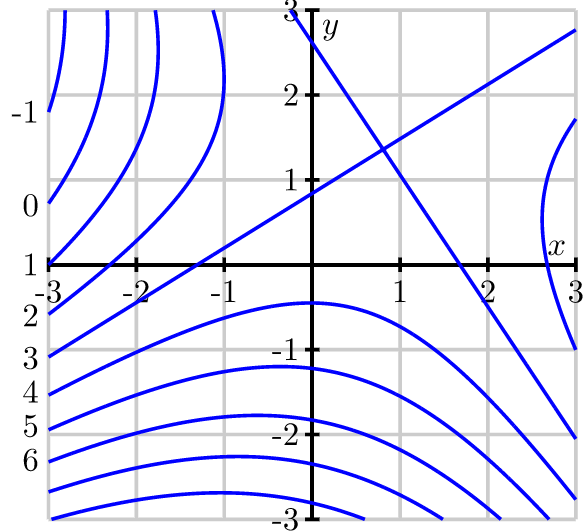
\includegraphics[width=0.5\textwidth]{203-keys/ps7-answer-key/10-2-6.png}
\end{center}
\begin{enumerate}
    \item Estimate the partial derivative $f_x(-2, -1).$
    
    \begin{red}
    We can use the contours to read off some approximate values and use a symmetric difference. 
    
    \textbf{NOTE:} I'm using a step size of 1 -- your answer may be a little different from this if you chose a different step size. Same deal in parts (b) and (c).
    \begin{align*}
        f(-3, -1) &\approx 3 \\
        f(-1, -1) &\approx 4.5 \\
        f_x(-2,-1) &\approx 
        \frac{f(-1, -1)-f(-3, -1)}{-1-(-3)} \\
        &= \frac{4.5-3}{2} = 0.75
    \end{align*}
    \end{red}
    
    \item Estimate the partial derivative $f_y(-2, -1).$
    
    \begin{red}
    Same game -- we can use the contours to read off some approximate values and use a symmetric difference: 
    \begin{align*}
        f(-2, -2) &\approx 6 \\
        f(-2, 0) &\approx 2.5 \\
        f_y(-2,-1) &\approx 
        \frac{f(-2, 0) - f(-2, -2)}{0-(-2)} \\
        &= \frac{2.5-6}{2} = -1.75
    \end{align*}
    \end{red}
    
    \item Estimate the partial derivatives $f_x(-1, 2)$ and $f_y(-1, 2)$.
    \begin{red}
    \begin{multicols}{2}
    \begin{align*}
        f(0, 2) &\approx 2.5\\
        f(-2, 2) &\approx 0.5 \\
        f_x(-1,2) &\approx 
        \frac{f(0,2)-f(-2,2)}{0-(-2)} \\
        &= \frac{2.5-0.5}{2} = 1
    \end{align*}
    
    \begin{align*}
        f(-1,1) &\approx 2.5 \\
        f(-1,3) &\approx 2.5 \\
        f_y(-1,2) &\approx
        \frac{f(-1,3)-f(-1,1)}{3-1} \\
        &= \frac{2.5-2.5}{2} = 0
    \end{align*}
    \end{multicols}
    \end{red}
    
    \item Locate, if possible, one point $(x,y)$ where $f_x(x,y)=0$.
    
    \begin{red}
    Looks like at about $(0, -0.5)$, if I move in the $x$ direction, the heights on the contour map don't change much.
    \end{red}
    
    \item Locate, if possible, one point $(x,y)$ where $f_x(x,y)<0$.
    
    \begin{red}
    Looks like at about $(1,-2)$, if I move in the $x$ direction, I'm going downhill.
    \end{red}
    
    \item Locate, if possible, one point $(x,y)$ where $f_y(x,y)>0$.
    
    \begin{red}
    Looks like at about $(1,2)$, if I move in the $y$ direction, I'm going (very slightly) uphill.
    
    \textbf{NOTE:} Of course there are other points that will work for all three of these parts.
    \end{red}

\end{enumerate}

\end{enumerate}


\end{document}